\subsection{Building a car}
The previous group had only built one car for their project. To show a situation where two cars meet at an intersection we needed to build a new car. Luckily, Accenture kept a box of unused components from the previous group. However, we only had one Tpu, the Coral Usb Accelerator. This was an important component for giving extra processing power to the computer, and it was necessary to run the artificial intelligence the previous group had used (source from previous project). 

Without this accelerator we could not run the artificial intelligence that the previous group had made. Due to the global chip shortage caused by the Covid pandemic, the accelerator was not available to purchase anywhere. This also made the camera and distance measuring sensor redundant, as these used artificial intelligence to process data. Not having two cars that utilized artificial intelligence could be a challenge, because one of the required features of our solution was that the cars should be able to override the server. We decided that as long as we had one car that could override the server commands the other car could drive solely on commands from the server. With the components, and the product documentation of the previous project (source from previous project), we were able to build a copy of the car.

\begin{figure}[h!]
	\centering
	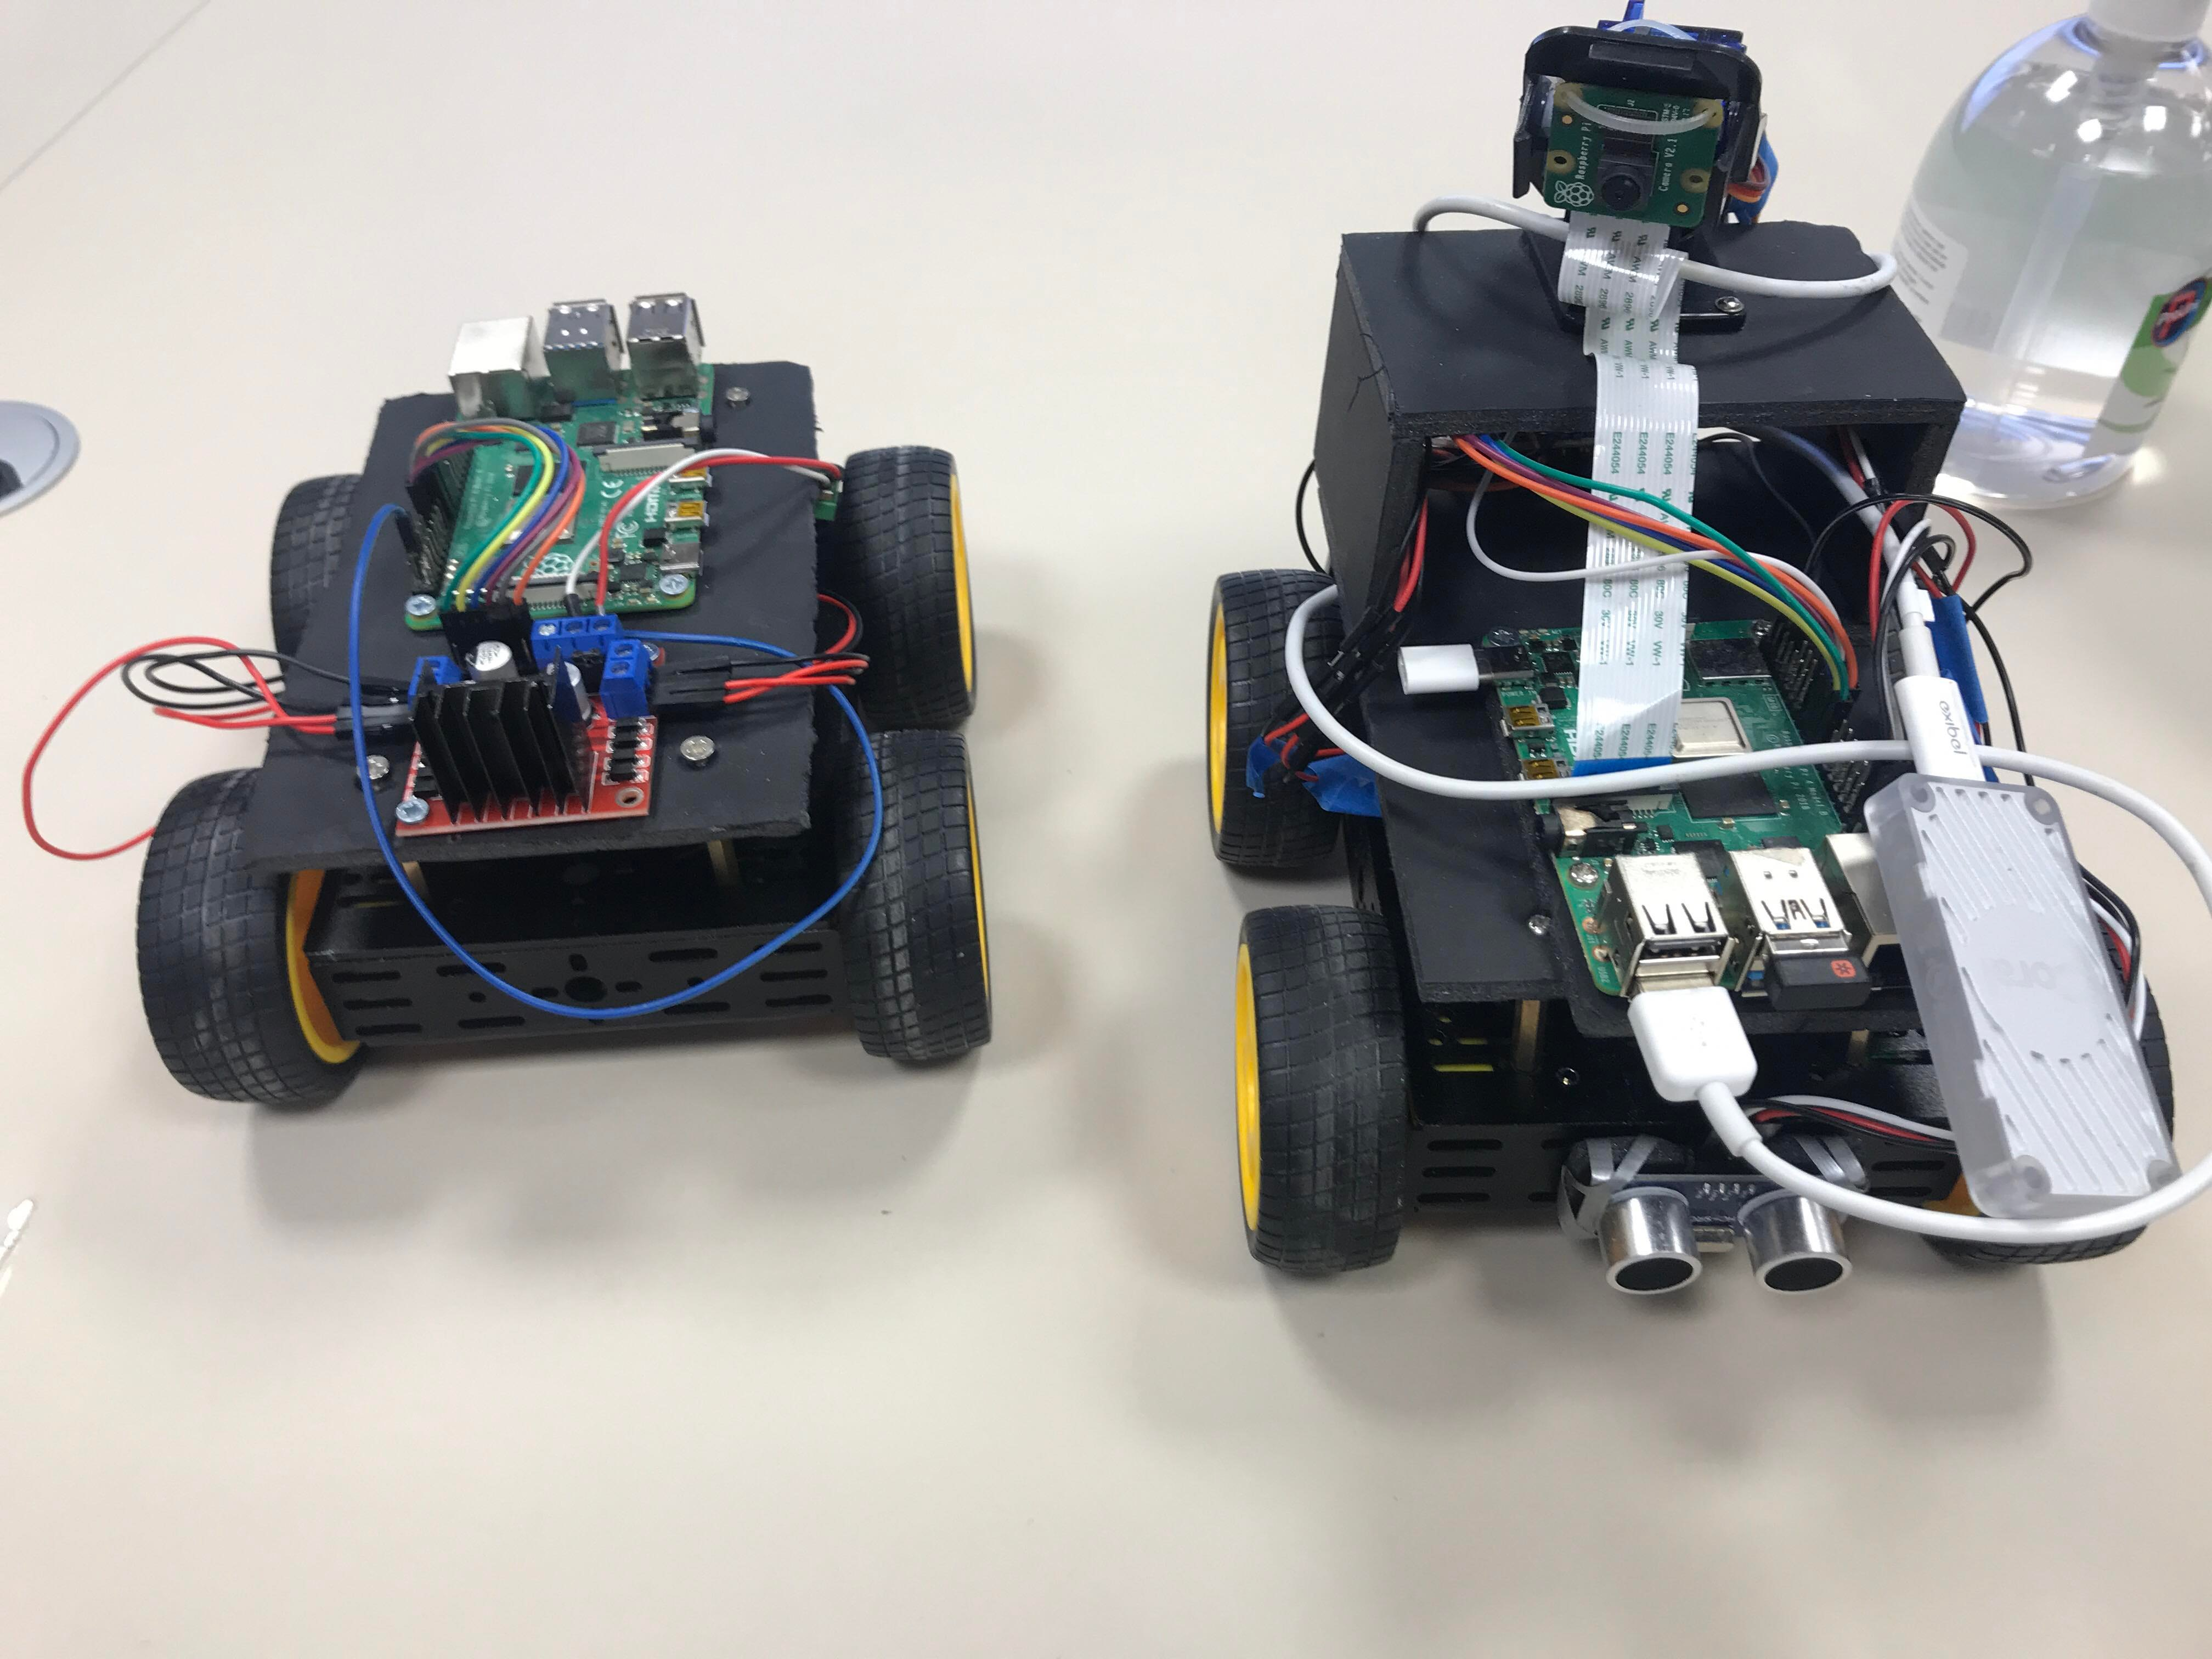
\includegraphics[width=1\linewidth]{figures/two_cars}
	\caption[scrum process]{Cars with and without camera, right to left}
	\label{fig:twocars}
\end{figure}



